\documentclass[conference]{IEEEtran}
\IEEEoverridecommandlockouts
\usepackage{cite}
\usepackage{amsmath,amssymb,amsfonts}
\usepackage{algorithmic}
\usepackage{graphicx}
\usepackage{textcomp}
\usepackage{booktabs}   % added: required by tab:splits and result tables
\usepackage{url}        % added: \url in bibliography (was missing upstream)
\usepackage{xcolor}
\def\BibTeX{{\rm B\kern-.05em{\sc i\kern-.025em b}\kern-.08em
    T\kern-.1667em\lower.7ex\hbox{E}\kern-.125emX}}
\begin{document}

\title{Structure-Preserving Style Augmentation for\\
Single-Source Cross-Domain Image Classification on PACS}

\author{\IEEEauthorblockN{Luoyu Liu}
\IEEEauthorblockA{2430033032}
\and
\IEEEauthorblockN{Member 2}
\IEEEauthorblockA{Student ID}
\and
\IEEEauthorblockN{Member 3}
\IEEEauthorblockA{Student ID}
\and
\IEEEauthorblockN{Member 4}
\IEEEauthorblockA{Student ID}
\and
\IEEEauthorblockN{Member 5}
\IEEEauthorblockA{Student ID}
}

\maketitle

\begin{abstract}
% TODO (Member 5)
Abstract to be written by member 5 after sections 1--5 stabilize.
\end{abstract}

\begin{IEEEkeywords}
domain generalization, style transfer, AdaIN, data augmentation, PACS
\end{IEEEkeywords}

%==================================================
\section{Introduction}
%==================================================

\subsection{Problem Statement}

A photo of a dog and a sketch of a dog share the label \texttt{dog}, yet they give a viewer very different clues. In the photo, fur texture, color, and lighting do most of the work. In the sketch, nearly all of that is gone, and the shape of the ears, the outline of the head, and the proportions of the body carry the identification. An image classifier that has learned to lean on photographic texture may therefore be lost when it meets a sketch of the very same animal. This mismatch between the visual features of training and test data is the \textit{domain shift} our project targets, and it is the core difficulty that domain generalization sets out to address~\cite{zhou2023dgsurvey}.

We ask two questions. First, if real photos are our only labeled training data, can style transfer help us generate training samples in many painting styles, and does that make a classifier better at recognizing paintings, cartoons, and sketches? Second, when we generate those samples, what if we adjust the \textit{style strength} locally according to image structure, so that regions such as object contours keep more of their original information? Would this produce better training data for cross-domain recognition than ordinary style transfer?

To answer both, we compare three training schemes on PACS. The first uses original photos only and serves as our baseline. The second adds images generated by adaptive instance normalization (AdaIN) to the same photos. The third adds images generated by structure-preserving style augmentation. All three use ResNet-18 and the same test lists. Comparing the first and second tells us what added style variety is worth. Comparing the second and third tells us whether protecting local structure brings an extra gain.

\subsection{Motivation and Background}

In supervised learning, data augmentation stretches a dataset by reshaping the samples we already have, giving each class more training examples. Flip a photo of a guitar and the body and neck swap sides, but it is still a \texttt{guitar}. This works as long as the transformed image keeps the visual evidence behind its original label. Flips and crops mostly change position, orientation, or what is in frame. The jump from photograph to painting also rewrites color, texture, and brushwork. That is why we turn to style transfer: it produces exactly the kind of appearance change our research question is about.

Prior work suggests this direction is promising. MixStyle starts from the observation that visual domain is closely tied to image style, as in photo versus sketch. By probabilistically mixing the feature statistics of training instances, it implicitly synthesizes new domains and improves generalization~\cite{zhou2021mixstyle}. Our setting differs in two ways. MixStyle mixes statistics across several source domains inside the network, whereas we have a single source domain and generate explicit stylized images from independent style references.

AdaIN takes a content image and a style image. In feature space, it shifts the mean and standard deviation of each content channel to match those of the style features, and a decoder then renders the result as an image~\cite{huang2017adain}. In our project, the training photo supplies the object and its label, while a separate style reference supplies the look. A guitar photo can be paired with a landscape painting. As long as the result still clearly shows a guitar, it becomes a valid new \texttt{guitar} training sample, and the painting never needs a \texttt{guitar} label.

This raises a question worth testing. Changing a guitar's color and surface texture exposes the model to more appearance variety. But if stylization melts a slender neck into the background, the new image inherits the \texttt{guitar} label while the shape cues that justify that label may have faded. Motivated by this, we use a structure map to guide local style strength, weakening the style where structural response is strong and keeping more of it elsewhere. Backgrounds can have sharp edges too, so the structure map is only an approximation of the class-relevant regions. Whether it helps must be judged by structural analysis of the generated images together with final cross-domain accuracy.

\subsection{PACS Dataset and Task Overview}

PACS contains four visual domains: Photo, Art Painting, Cartoon, and Sketch. Each domain covers the same seven object classes: \texttt{dog}, \texttt{elephant}, \texttt{giraffe}, \texttt{guitar}, \texttt{horse}, \texttt{house}, and \texttt{person}. The classification goal stays fixed while the way objects are depicted changes, which lets us see how a model copes with different styles~\cite{li2017dg}.

\begin{figure}[t]
\centering
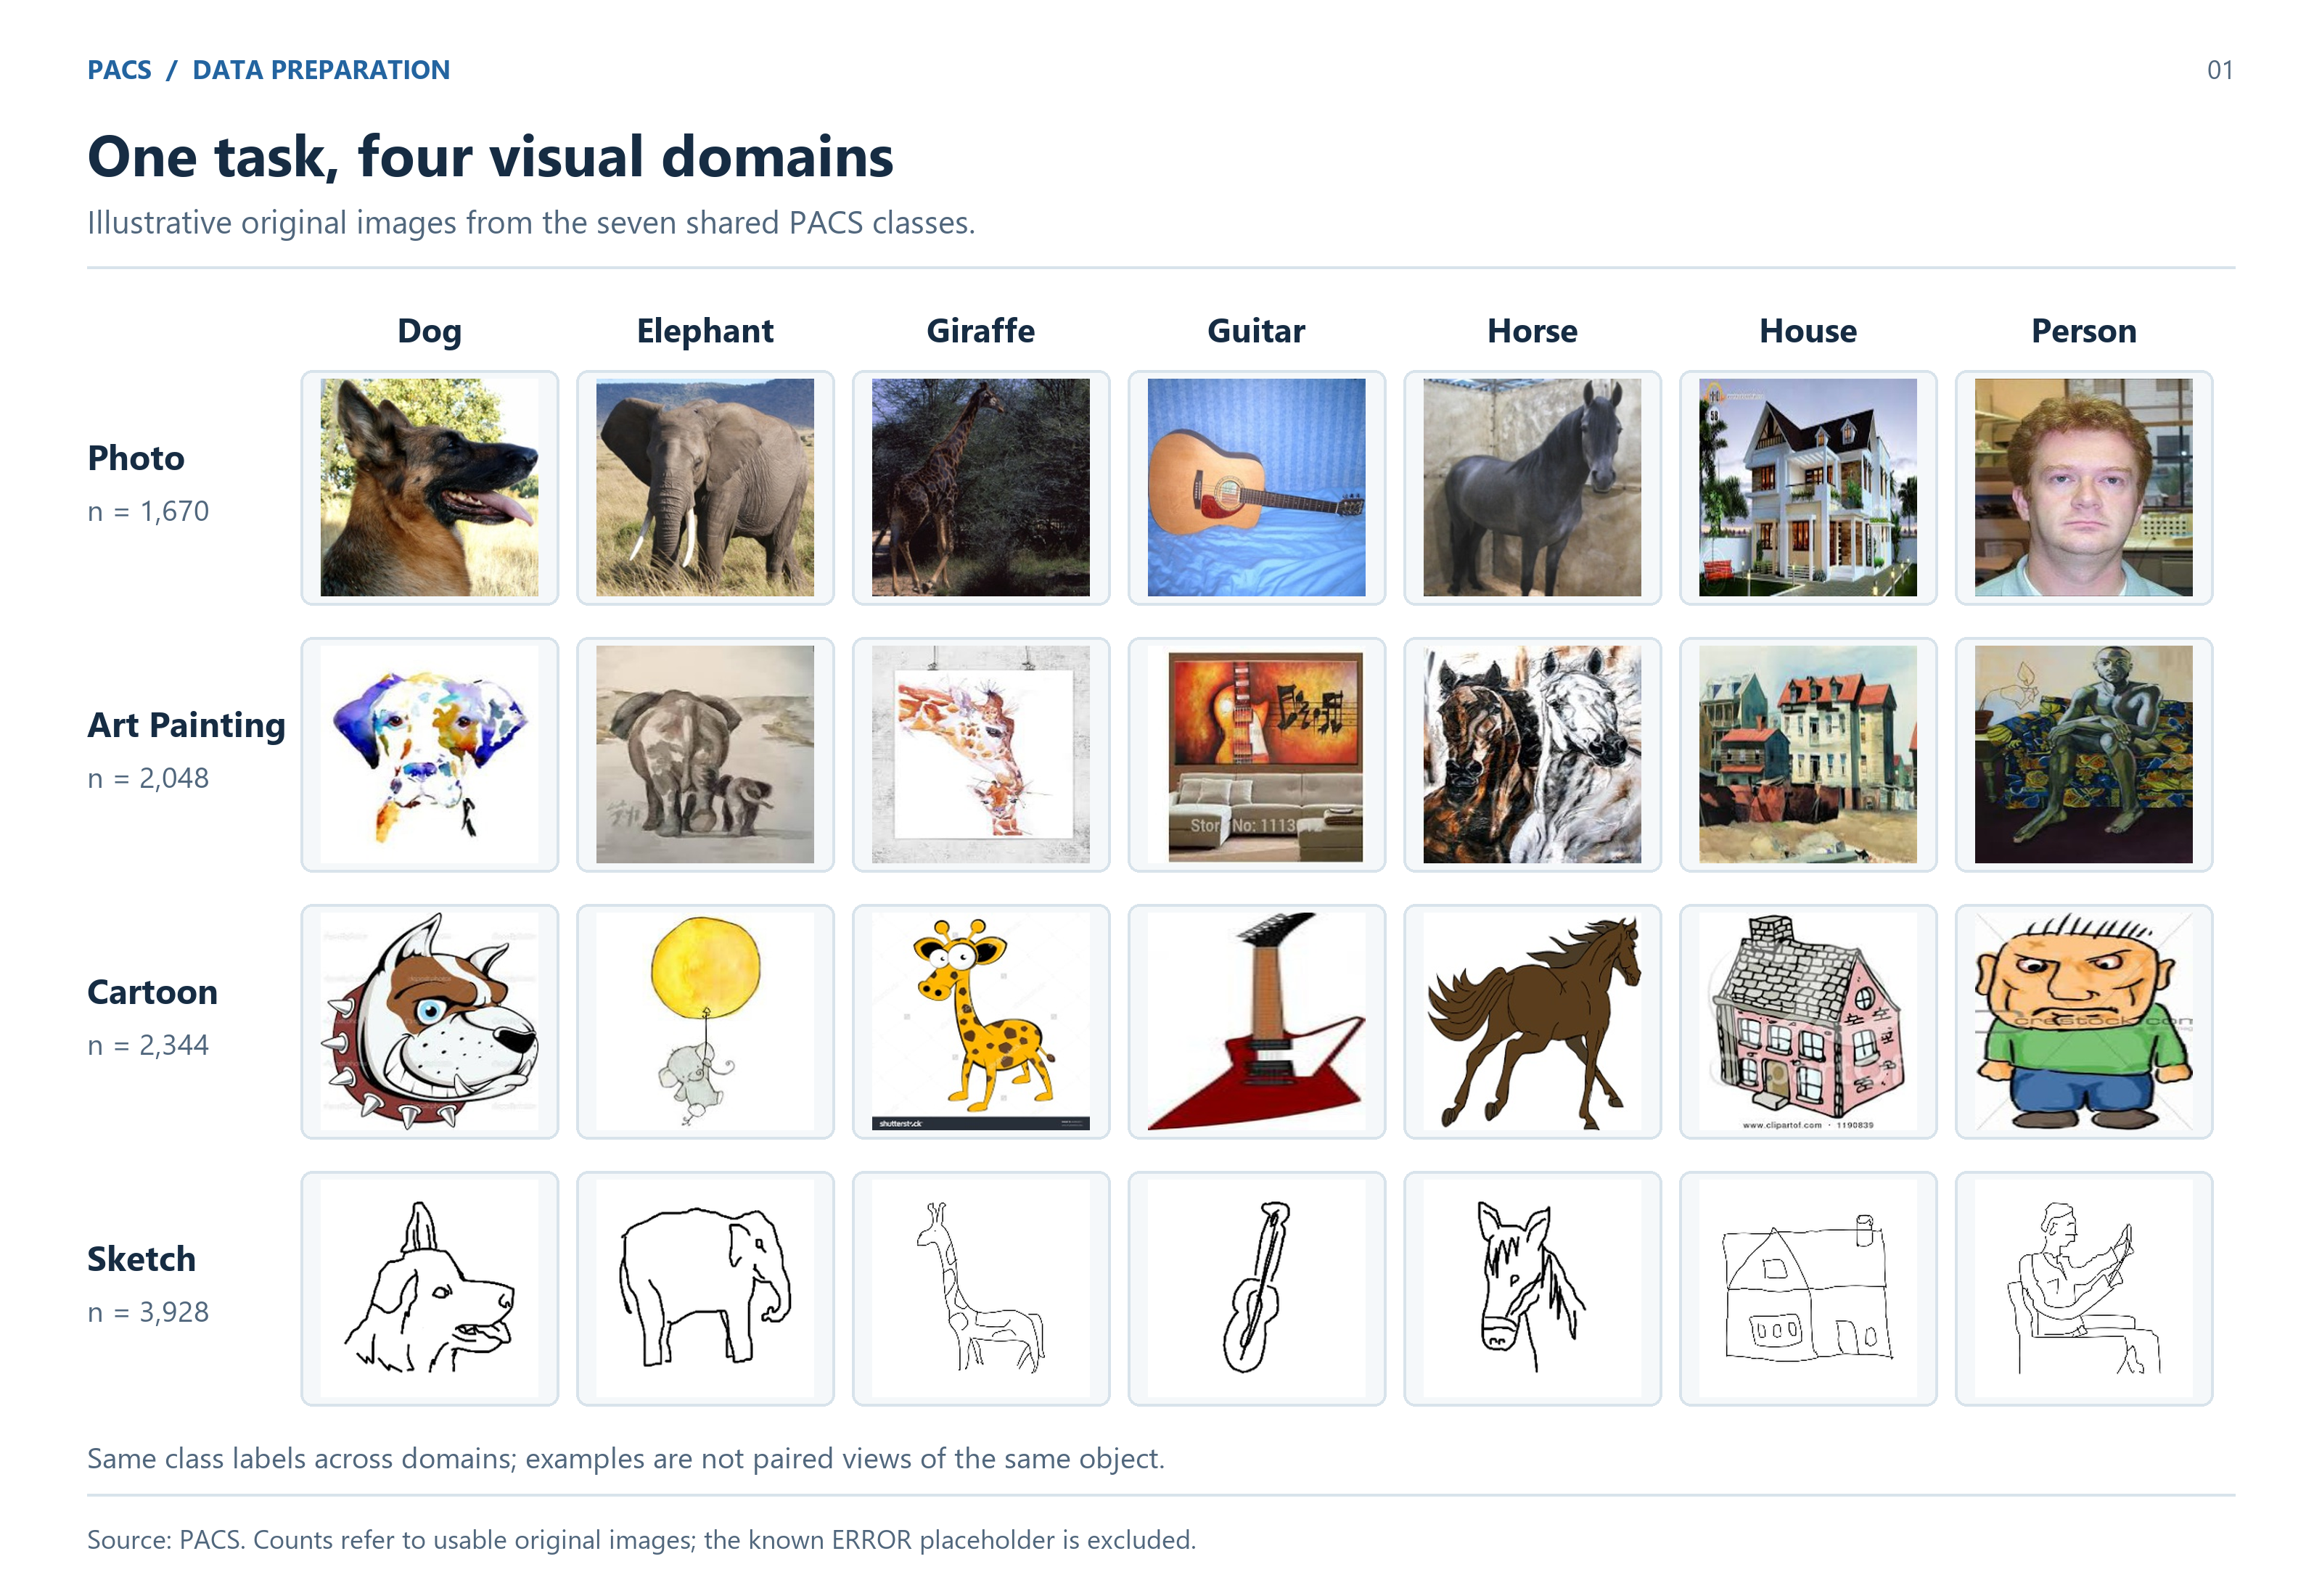
\includegraphics[width=\columnwidth]{figures/1.3_PACS四域七类样例图.png}
\caption{Illustrative examples from PACS. Rows correspond to visual domains and columns to object classes. Images in the same column are independent examples of the same class.}
\label{fig:pacs_examples}
\end{figure}

Follow the \texttt{guitar} column in Fig.~\ref{fig:pacs_examples}. The photo shows the material and lighting of the instrument, the cartoon uses flat color blocks and exaggerated shapes, and the sketch relies almost entirely on lines for the body and neck. Each row holds independent PACS samples. What a column shares is the class, not a paired image of the same object.

We use Photo as the source domain. During training, we read labeled photos from Photo Training and generate stylized samples from them. At test time, we classify the original PACS images in Art Painting, Cartoon, and Sketch. This separation matters. A painting-style image generated from a training photo may enter the training set, but the PACS Art Painting images used for final evaluation always stay in the test set. The style references that produce those training images are themselves drawn from outside PACS, so no evaluation image reaches the training set either through the content or through the style. We also hold out a set of Photo images to see how the classifier performs on original photos.

%==================================================
\section{Related Work}
%==================================================

\subsection{Cross-Domain Image Classification and PACS}

Cross-domain image classification studies what happens when training and test data come from different domains. With shared classes, the question the model answers is the same at training and test time, for instance ``is this a guitar?'', but the visual features it can rely on shift with the domain. Domain generalization goes one step further. It aims to learn from source domains alone and perform well on unseen ones, so the target domain must stay out of model development and serve only as independent evaluation~\cite{zhou2023dgsurvey}. Existing methods span domain alignment, meta-learning, data augmentation, and ensemble learning, and our work falls in the data augmentation family.

Li \textit{et al.} introduced PACS, bringing real photos, art paintings, cartoons, and sketches into a single domain generalization benchmark. Their original protocol is multi-source. Each round uses three domains for training and leaves the fourth for testing. With Sketch as the target, for example, the model can train on Photo, Art Painting, and Cartoon together. The aim is to test whether a model can learn recognition features from several seen domains that also work on a different one~\cite{li2017dg}. Later work has used PACS to study how style affects generalization. MixStyle, for example, shows that photo, art painting, cartoon, and sketch images are well separated in the space of feature statistics, and it uses this to synthesize new domains~\cite{zhou2021mixstyle}.

We keep PACS's classes and domain definitions and adopt a \textit{single-source Photo-only} setting. ``Photo-only'' means the labeled original training content comes entirely from Photo. Both style augmentation methods draw on a frozen pool of 10 external paintings for style references, none of which belongs to PACS; PACS target-domain test images never take part in generating training samples, choosing parameters, or updating the model. We chose this setting to isolate one factor: with the labeled photos fixed, how does changing their style, and protecting structure while doing so, affect cross-domain recognition? Because the information available at training time differs from multi-source protocols, we judge our methods by comparing the three groups under the same Photo-only setting.

% TODO (Member 2): \subsection{Style Transfer and AdaIN}
% TODO (Member 2): \subsection{Style Augmentation for Image Classification}
% TODO (Member 3): \subsection{Structure Preservation and Structure-Related Metrics}

%==================================================
\section{Method}
%==================================================

% Member 4 - Section 3.1 Overall Framework
\subsection{Overall Framework}
\label{sec:overall_framework}

Fig.~\ref{fig:framework} summarizes the pipeline. All three experimental groups share one architecture, one set of data splits, and one evaluation protocol, and differ in exactly one factor: the set of images used for training.

\begin{figure}[t]
\centering
% Overall framework diagram. Source: figures/framework.mmd (Mermaid).
% Render with:  npx -y @mermaid-js/mermaid-cli -i figures/framework.mmd -o figures/framework.pdf -b white -s 2
% If the PDF is absent, fall back to the PNG, and finally to a placeholder.
\IfFileExists{figures/framework.pdf}{%
  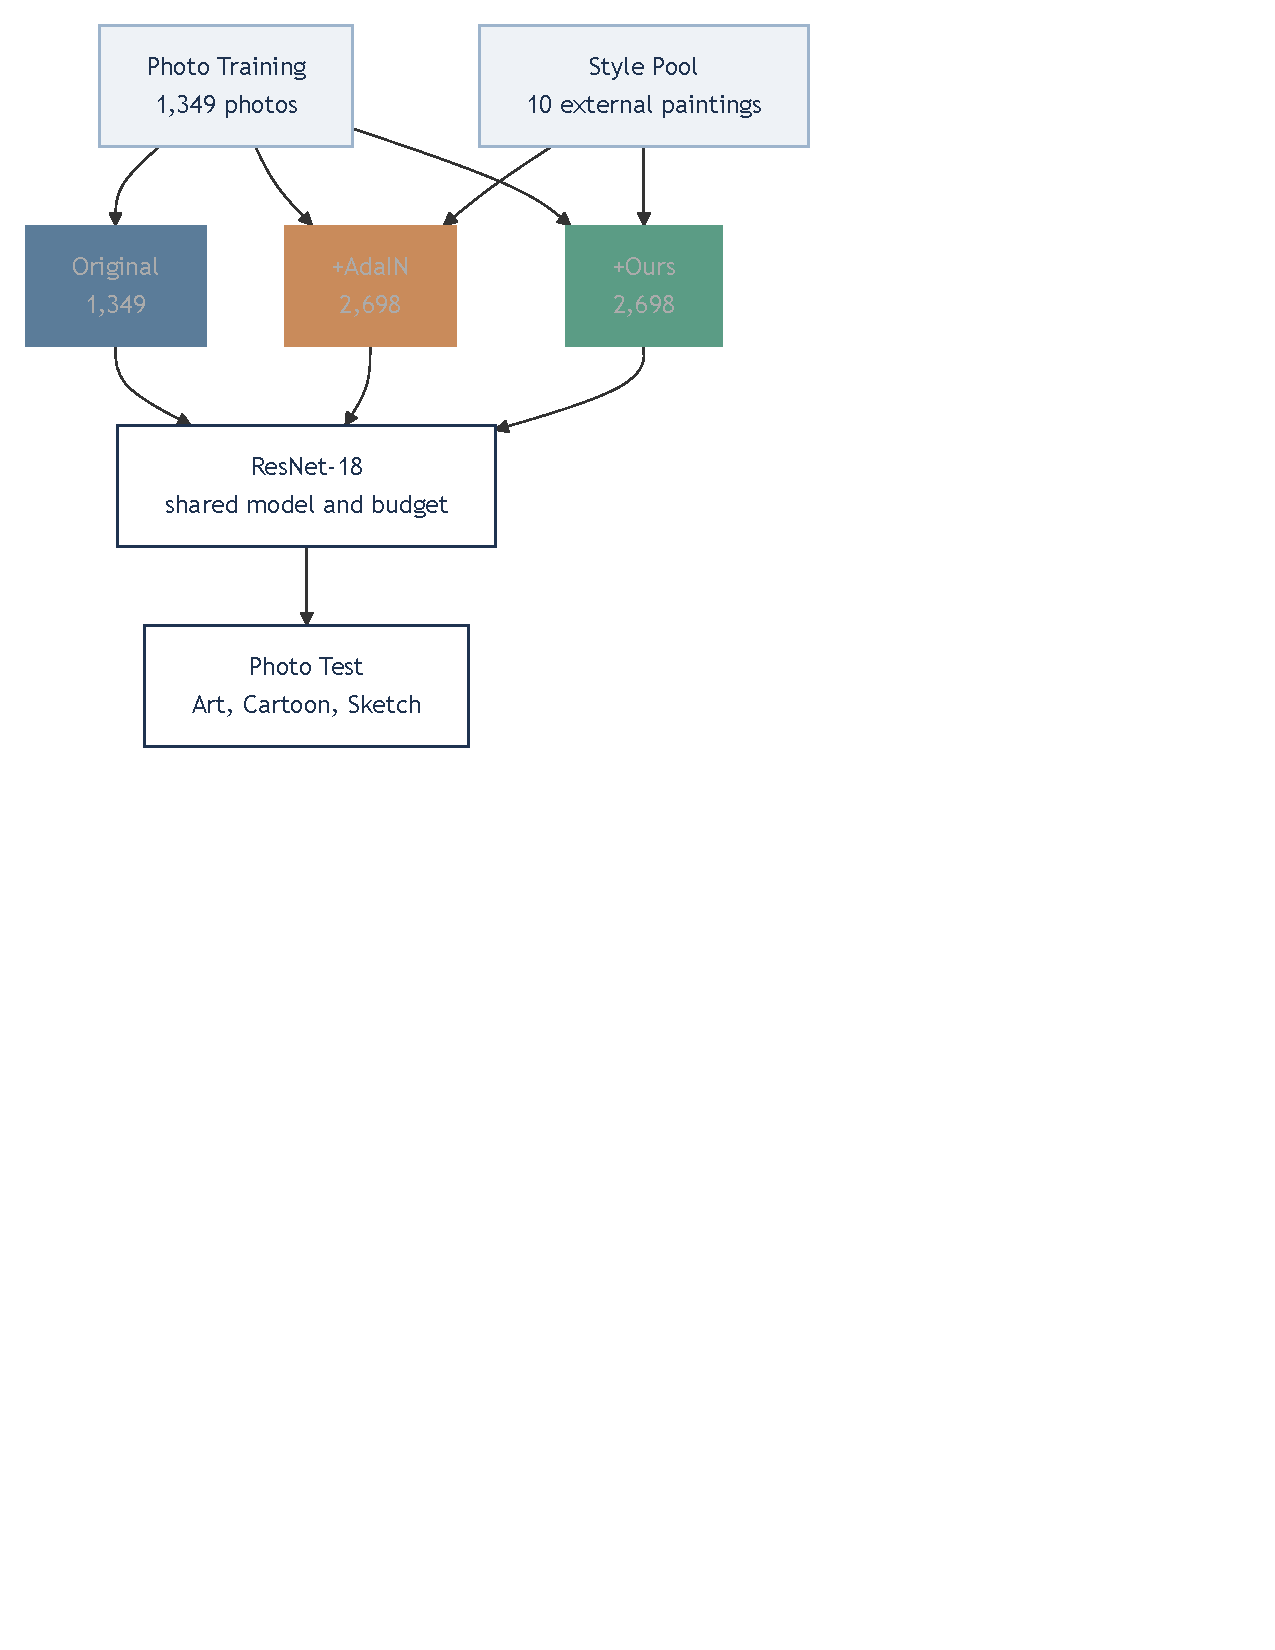
\includegraphics[width=\columnwidth]{figures/framework.pdf}%
}{%
  \IfFileExists{figures/framework.png}{%
    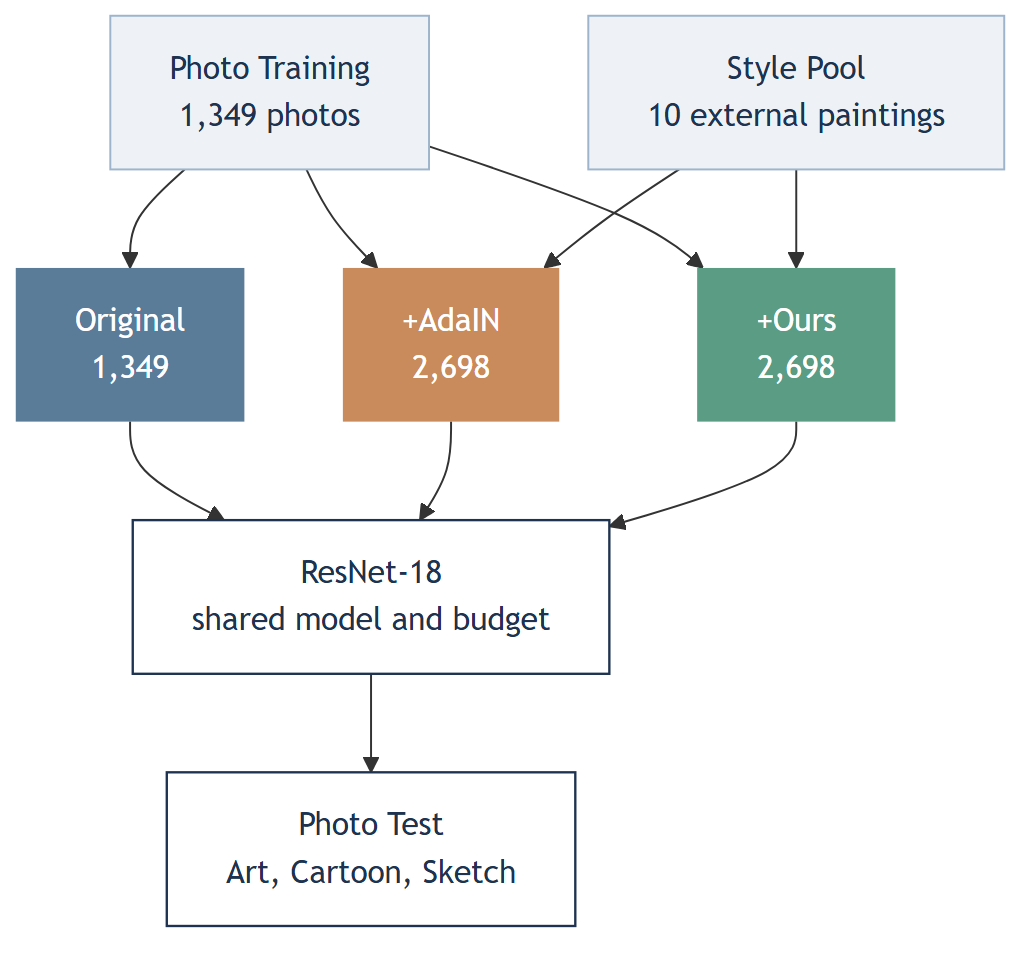
\includegraphics[width=\columnwidth]{figures/framework.png}%
  }{%
    \fbox{\parbox[c][2.2cm][c]{\dimexpr\columnwidth-2\fboxsep-2\fboxrule\relax}{\centering Placeholder: overall framework figure (planned).}}%
  }%
}
\caption{Overall framework. Photo Training images feed three training sets: originals only, originals plus AdaIN stylizations, and originals plus structure-preserving stylizations. Both stylized sets draw their style references from one frozen pool of external paintings. A single ResNet-18 training and evaluation protocol is applied to all three groups.}
\label{fig:framework}
\end{figure}

Stylized training images are produced \textit{offline}. Member 2's AdaIN generator and member 3's structure-preserving generator each write images to disk together with a manifest that records the content image, the style image, the style strength $\alpha$, and, for the structure-preserving variant, the structure parameter $\beta$. Training then reads from these fixed manifests, so the three groups go through an identical data-loading path. Nothing about the stylization is recomputed or resampled during classifier training, which keeps the classifier-side training code common to all groups.

Table~\ref{tab:groups} defines the three groups. The comparison Original vs.\ +AdaIN isolates the value of added style diversity (experiment 2), and +AdaIN vs.\ +Ours isolates the value of structure preservation (experiment 3), as detailed in Section~\ref{sec:exp_design}.

\begin{table}[t]
\caption{The three training groups. All groups use the same splits, model, and evaluation.}
\label{tab:groups}
\centering
\small
\setlength{\tabcolsep}{4pt}
\begin{tabular}{@{}lrr@{}}
\toprule
Group & Training images & Composition \\
\midrule
Original & 1{,}349 & Photo Training only \\
+AdaIN   & 2{,}698 & $+ 1{,}349$ AdaIN \\
+Ours    & 2{,}698 & $+ 1{,}349$ structure-preserving \\
\bottomrule
\end{tabular}
\end{table}

\subsection{Dataset and Task Definition}

We define the task as seven-class supervised image classification. Given one input image, ResNet-18 must predict one of the seven PACS object classes. In the style augmentation experiments, style images are used only to construct training data. At classification time, the model sees a single image.

\textit{Dataset size and class distribution.} Our local copy of PACS holds 9,991 images, all of which decode correctly. One image under \texttt{Sketch/dog} actually displays the word ``ERROR''. Based on its content and the PACS loading rules in Dassl~\cite{zhou2020dassl}, we excluded it from our lists. The remaining 9,990 images comprise 1,670 Photo, 2,048 Art Painting, 2,344 Cartoon, and 3,928 Sketch images. Fig.~\ref{fig:pacs_counts} shows the actual count of each of the seven classes in every domain, before any style augmentation.

\begin{figure}[t]
\centering
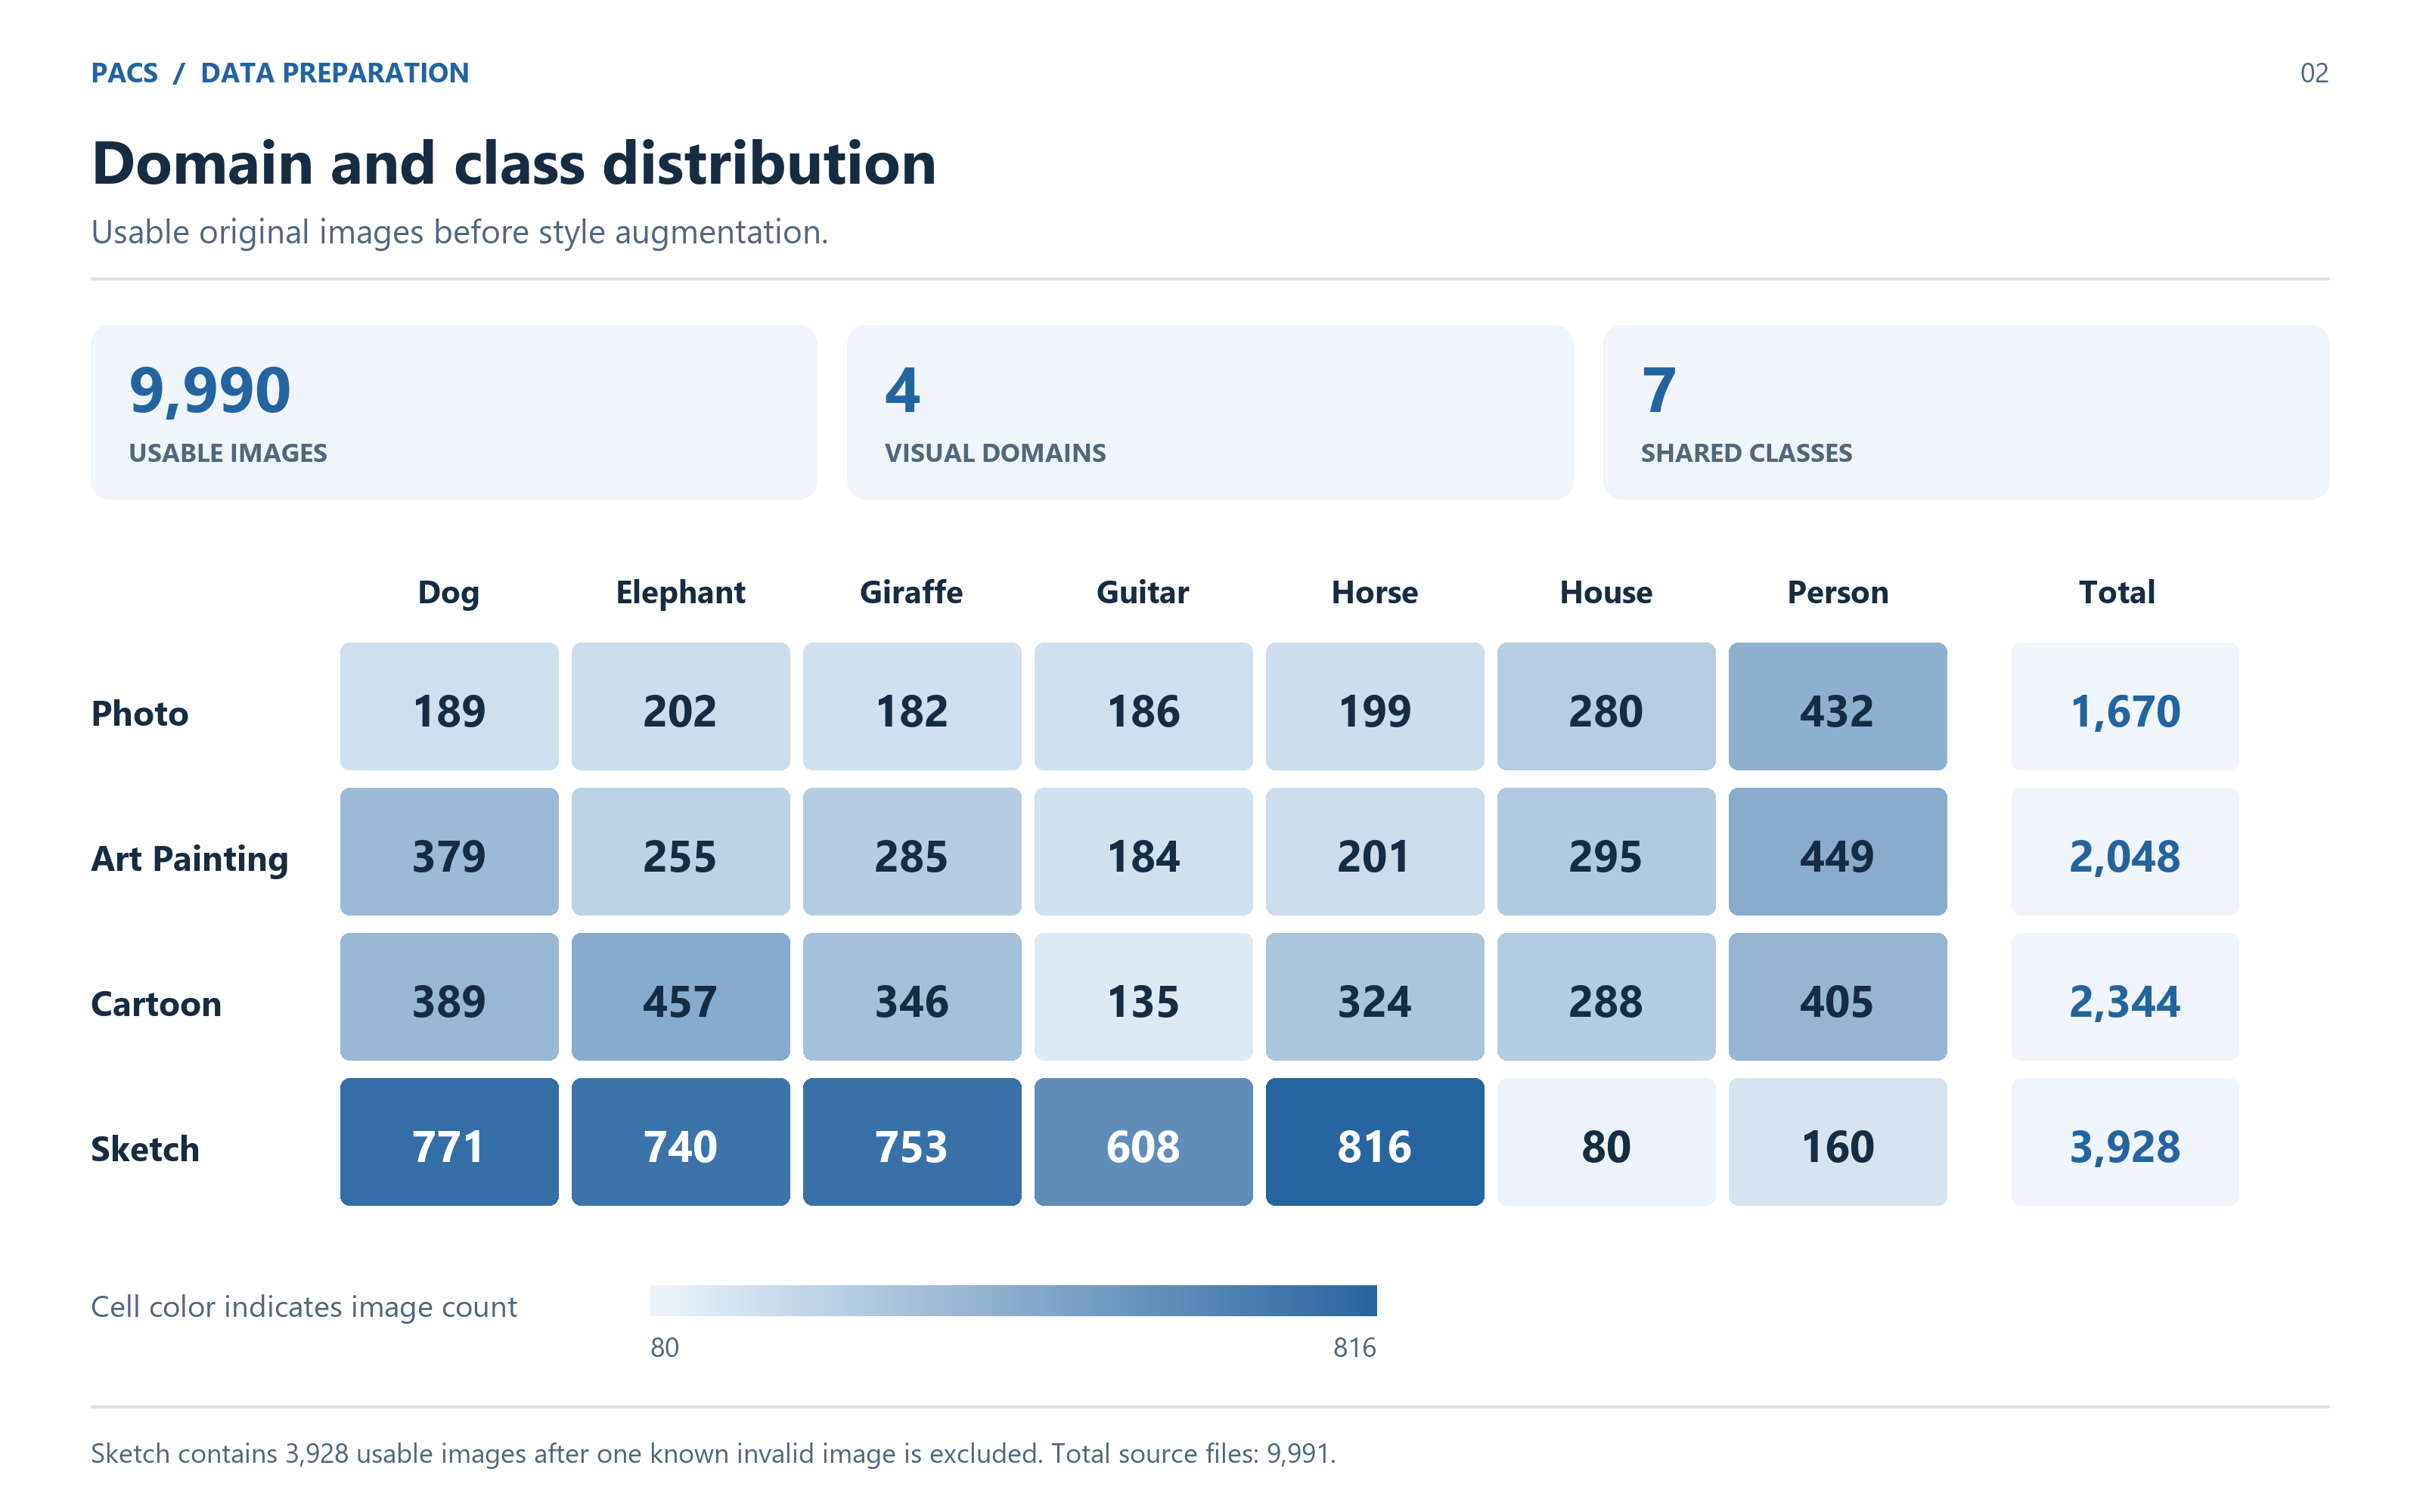
\includegraphics[width=\columnwidth]{figures/3.2_PACS各域类别数量统计图.png}
\caption{Number of usable PACS images by domain and class before style augmentation.}
\label{fig:pacs_counts}
\end{figure}

\textit{Source domain split.} The original \texttt{photo\_train\_kfold.txt} lists 1,499 photos and \texttt{photo\_crossval\_kfold.txt} lists another 171. The original \texttt{photo\_test\_kfold.txt} lists all 1,670 photos, overlapping with the first two. To obtain an independent in-domain evaluation, we keep the 171 photos from the original \texttt{crossval} list as our final Photo Test. From the 1,499 photos in the original \texttt{train} list, we apply stratified sampling by class with random seed 42 and hold out about 10\% of each class for validation. This yields 1,349 Photo Training images and 150 Photo Validation images.

\textit{Target domains and how each split is used.} All usable images from Art Painting, Cartoon, and Sketch form three separate target-domain test sets. Every model uses the same lists, as summarized in Table~\ref{tab:splits}.

\begin{table}[t]
\caption{Data splits and their experimental roles.}
\label{tab:splits}
\centering
\small
\begin{tabular}{@{}lrp{4.4cm}@{}}
\toprule
Split & Images & Purpose \\
\midrule
Photo Training    & 1,349 & Update classifier parameters; provide labeled content images for augmentation \\
Photo Validation  & 150   & Select parameters and model checkpoints \\
Photo Test        & 171   & Measure in-domain accuracy \\
Art Painting Test & 2,048 & Measure cross-domain accuracy on art paintings \\
Cartoon Test      & 2,344 & Measure cross-domain accuracy on cartoons \\
Sketch Test       & 3,928 & Measure cross-domain accuracy on sketches \\
\bottomrule
\end{tabular}
\end{table}

\begin{figure}[t]
\centering
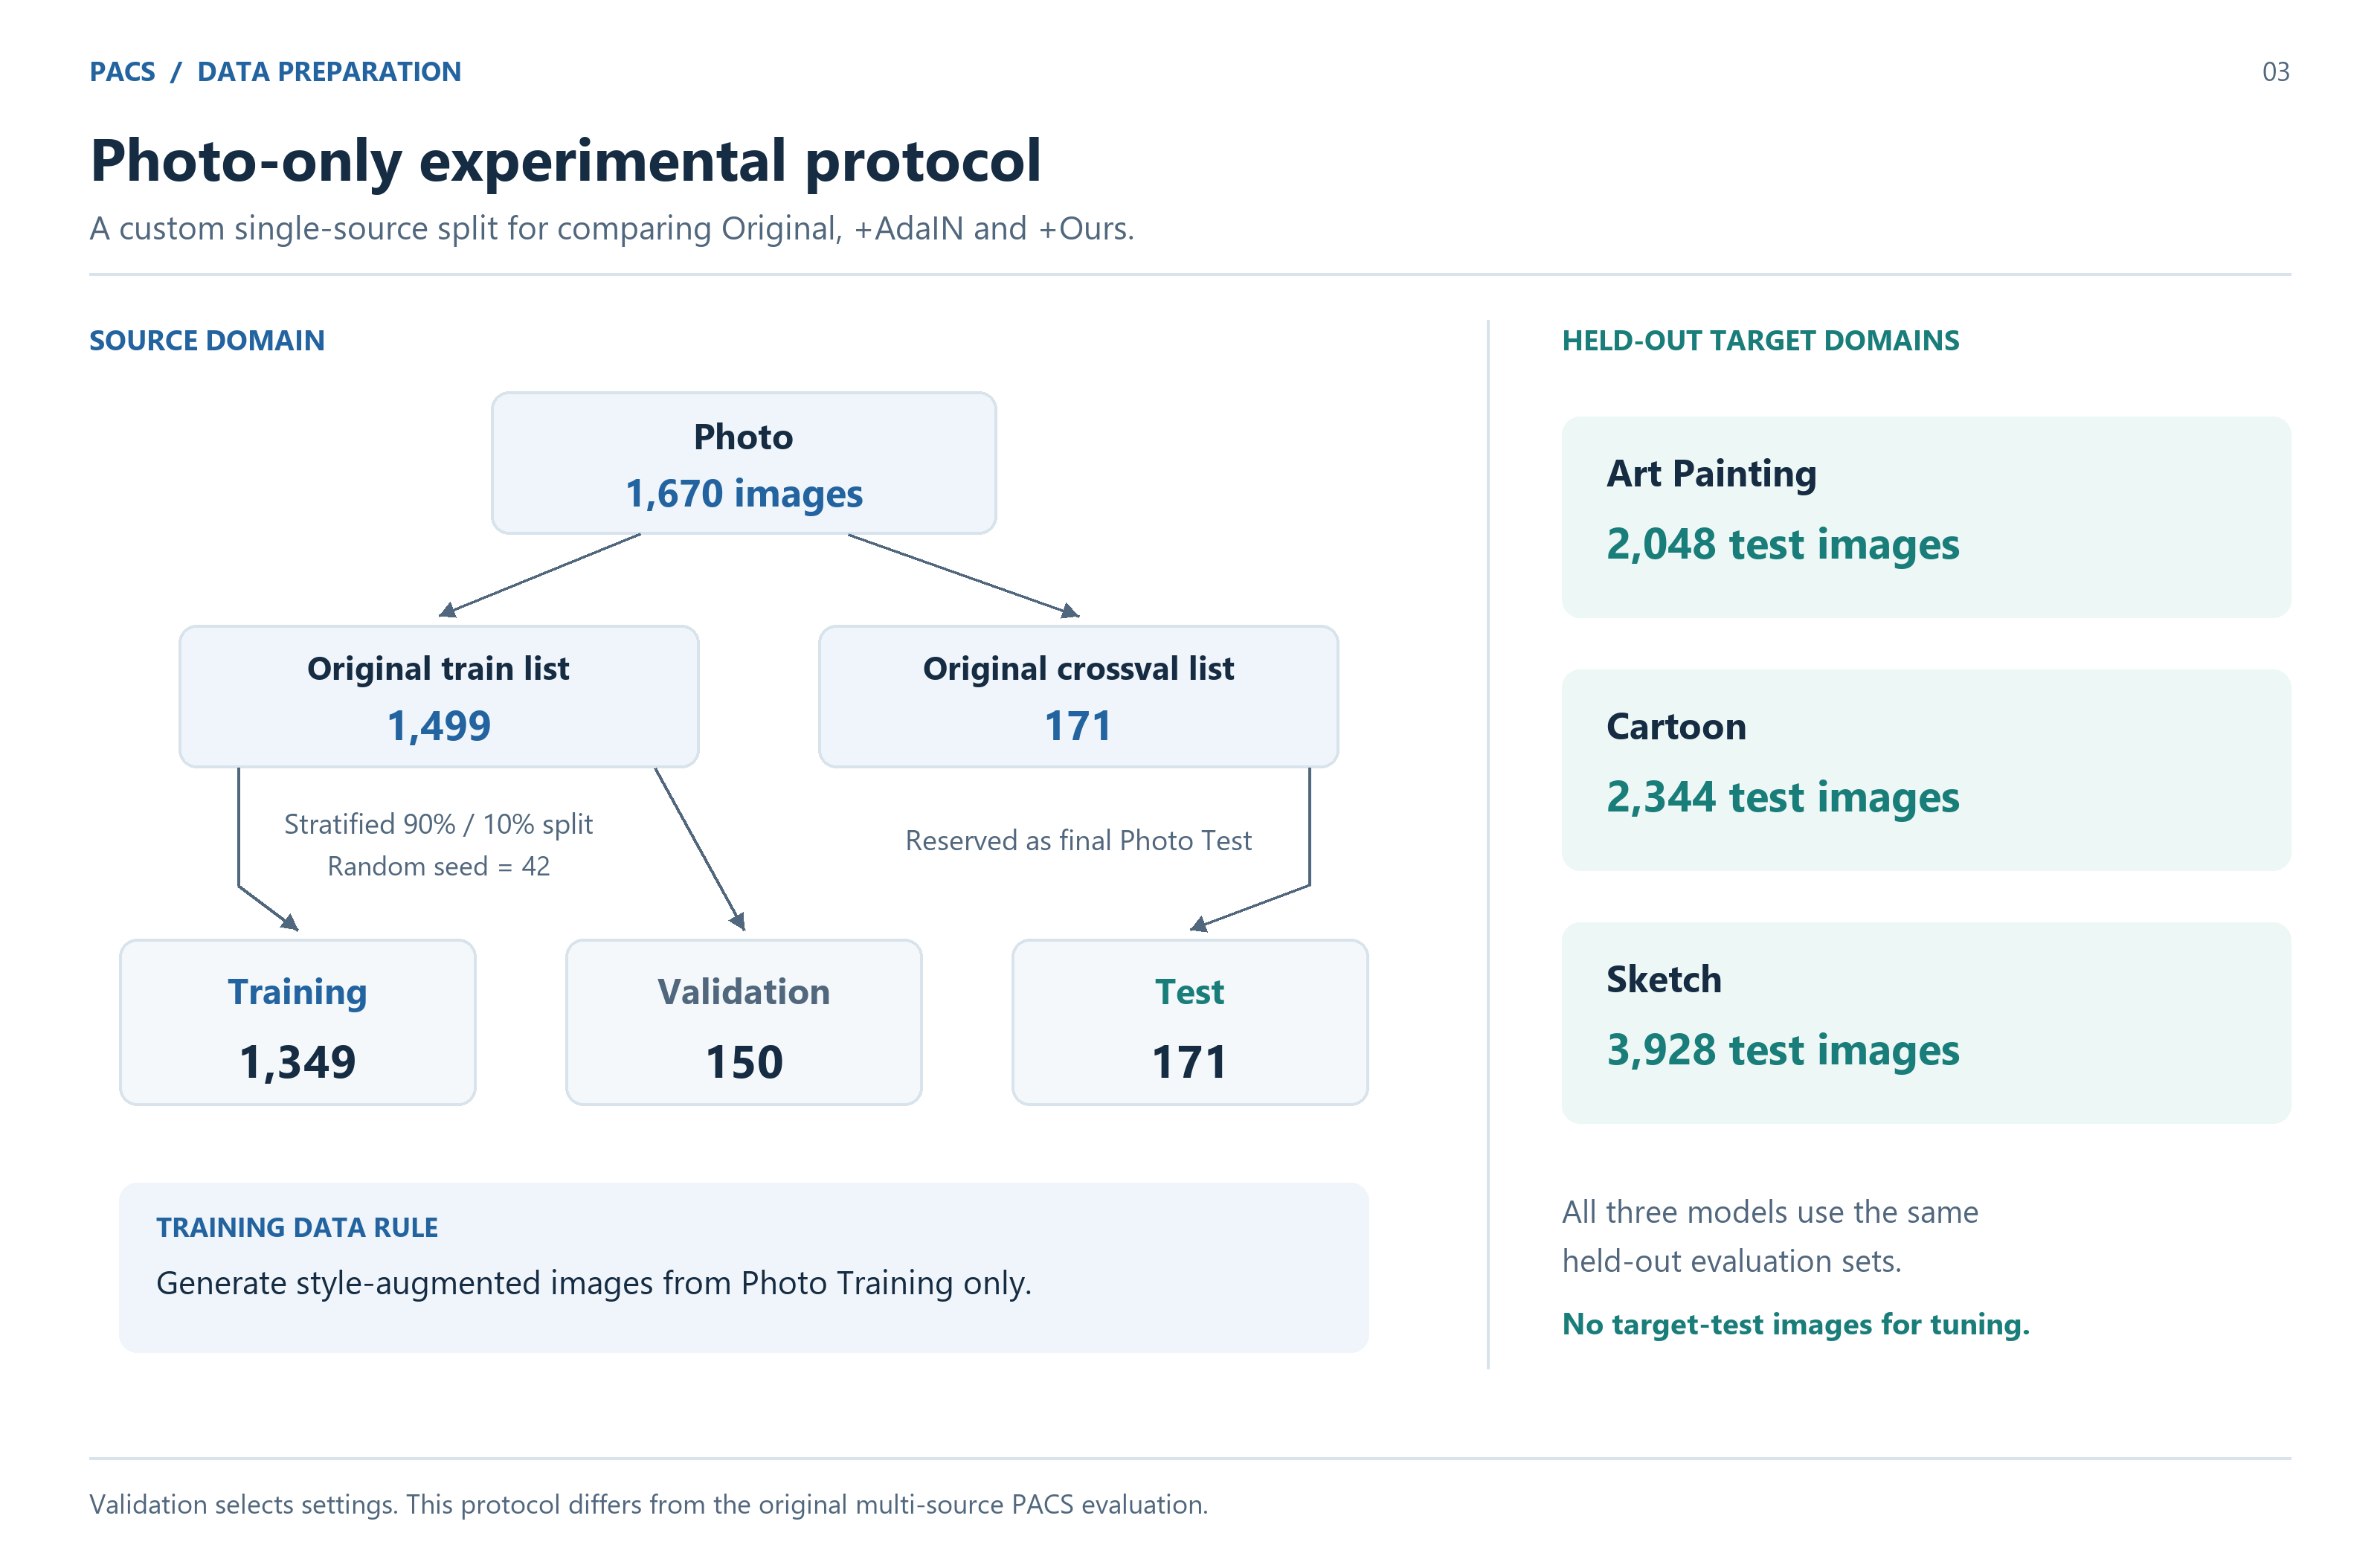
\includegraphics[width=\columnwidth]{figures/3.2_数据划分与实验任务流程图.png}
\caption{Photo-only experimental protocol. The training images provide content for style augmentation. The Photo test set and the three target-domain test sets are held out for final evaluation.}
\label{fig:split_protocol}
\end{figure}

\textit{Data rules for the three experimental groups.} The Original group trains on the 1,349 original Photo Training images. The +AdaIN group adds images generated by standard AdaIN, and the +Ours group adds images from structure-preserving style augmentation. Both augmented groups share the same original photos, the same style pool, and the same number of augmented samples. Each generated image inherits the label of its content image. All augmentation happens after the data split and draws content only from Photo Training (Fig.~\ref{fig:split_protocol}). The style pool is a frozen set of 10 external paintings that are not part of PACS. Because Art Painting, Cartoon, and Sketch are our evaluation domains, style references are taken from outside the dataset entirely, and the checker verifies mechanically that no style image is a PACS image; otherwise the test appearance would reach the training set through the stylization step.

Together, the six project lists cover all 9,990 usable images. We verified that no path appears in more than one list, and found no cross-split images with identical file contents or identical decoded pixels. For the final evaluation, we report classification accuracy separately on Art Painting, Cartoon, and Sketch to see how style augmentation affects each target domain. Photo Test accuracy serves as a supporting metric, showing whether changes in cross-domain performance come with changes in recognition of original photos.

% Member 4 - Section 3.3 ResNet-18 Baseline
\subsection{ResNet-18 Baseline}
\label{sec:resnet_baseline}

We use ResNet-18~\cite{he2016resnet} as the classifier for all groups. It is the standard backbone for PACS-style domain generalization studies, and its moderate size fits our single-GPU compute budget while leaving room for multi-seed replication.

The network is initialized with ImageNet-pretrained weights, and the final fully connected layer is replaced with a seven-way classifier head. All layers are fine-tuned jointly. Pretraining matters in our setting: Photo Training has only 1{,}349 images, and training the same architecture from scratch on this amount of data yields a weak baseline that would compress the dynamic range of all comparisons.

\textit{Input transforms.} Training uses RandomResizedCrop to $224\times224$ with scale $(0.7, 1.0)$ and a horizontal flip, followed by ImageNet normalization. Evaluation resizes the shorter side to 256, center-crops to $224\times224$, and applies the same normalization. We deliberately exclude photometric augmentation such as color jitter and grayscale: those transformations change style-related statistics, which is exactly the variable under study, so adding them to all groups would confound the comparison. Geometric augmentation only is applied, identically in all groups.

\textit{Optimization.} All groups are trained with SGD (momentum 0.9, weight decay $5\times10^{-4}$, label smoothing 0.1~\cite{szegedy2016rethinking}), initial learning rate 0.01, batch size 64, and a cosine schedule~\cite{loshchilov2017sgdr} over a fixed step budget of 660 optimizer steps (Section~\ref{sec:exp_design}). We report the \textit{final} checkpoint of that budget, with no checkpoint selection on any validation split: we measured that selecting on Photo Validation accuracy inflates the seed-to-seed spread of cross-domain accuracy, and the measurement is reported in Section~\ref{sec:training_prep}. Target-domain test sets never influence training, checkpoint selection, or any hyperparameter choice.

% TODO (Member 2): \subsection{AdaIN Style Augmentation}
% TODO (Member 3): \subsection{Structure-Preserving Style Augmentation}

% Member 4 - Section 3.6 Evaluation Metrics
\subsection{Evaluation Metrics}
\label{sec:evaluation_metrics}

\textit{Classification accuracy.} We report top-1 accuracy on Photo Test (in-domain) and on each of Art Painting, Cartoon, and Sketch (cross-domain). The primary metric is the unweighted average of the three cross-domain accuracies. Every configuration is run with three training seeds; we report mean and standard deviation over seeds, and per-domain breakdowns are included so that effects which appear in only one domain are visible.

\textit{Structure preservation.} To characterize the generated data rather than the classifier, we compare each stylized image with its content image using two measures. The first is LPIPS~\cite{zhang2018lpips}, a perceptual distance between the two images; larger values mean the stylization moved the image further from its content. The second is \textbf{EdgeScore}, an edge-consistency measure built from Canny edge maps~\cite{canny1986}. Writing $E_c$ and $E_s$ for the binary edge maps of the content and the stylized image, we report

\[
\text{EdgeScore} = \frac{2PR}{P+R}, \quad
P = \frac{|E_c \cap E_s|}{|E_s|}, \quad
R = \frac{|E_c \cap E_s|}{|E_c|},
\]

which is the F1-style overlap of the two edge maps: it is 1 when the stylized image reproduces all of the content's contours and falls as the stylization erases them. Note that this is an \textit{overlap}, not a difference: it is the harmonic mean of the fraction of stylized edges that coincide with a content edge (precision) and the fraction of content edges that survive in the stylized image (recall). A plain edge difference would score a stylization that adds many spurious edges but keeps the content's contours as poorly as one that erases them, whereas EdgeScore rewards agreement in both directions. Canny thresholds are held fixed across all images so that scores are comparable. These metrics describe how much structure the generated data removes; they are analysis metrics and do not enter training or model selection.

% Member 4 - Section 3.7 Experimental Design and Fair Comparison
\subsection{Experimental Design and Fair Comparison}
\label{sec:exp_design}

\textit{Experiments.} Four experiments answer the four research questions in the Introduction. Experiment 1 trains the Original group and measures the Photo-versus-target gap. Experiment 2 compares Original against +AdaIN. Experiment 3 compares +AdaIN against +Ours with everything else held fixed. Experiment 4 sweeps the style strength $\alpha \in \{0.25, 0.5, 0.75, 1.0\}$ for both augmentation methods, tracing the relation between stylization strength, structure preservation, and cross-domain accuracy. A $\beta$ ablation for the structure-preserving method is planned alongside Experiment 4 (Section~5.3).

\textit{Fairness controls.} Because the compared methods differ only in their training images, the following quantities are fixed across groups:

\begin{itemize}
\item \textit{Same original data:} all groups train on the identical 1{,}349 Photo Training images from Table~\ref{tab:splits}.
\item \textit{Same style pool:} both augmented groups draw style references from one frozen pool of 10 style images, fixed with a content-hash manifest before any training run. The pool holds external paintings that are not part of PACS, and the checker verifies this mechanically (the ``No test-set leakage'' item below).
\item \textit{Same augmentation count:} each augmented group adds exactly one stylized image per original training image (1{,}349 added images).
\item \textit{Same content--style pairing:} the style image paired with each content image is drawn once with a fixed seed and reused by both generators, so the only difference between the two augmented datasets is the stylization algorithm itself.
\item \textit{Same transform pipeline and classifier:} one training script, one transform definition, one ResNet-18 configuration for all groups.
\item \textit{Same optimization budget:} all groups receive the same number of optimizer steps, $S = 660$, computed as 30 passes over the Original training set at batch size 64 ($30 \times 22$). Groups with larger training sets accordingly run fewer passes over their data. Validation is evaluated at the same step cadence for every group.
\item \textit{Same evaluation and seeds:} all groups use the test lists of Table~\ref{tab:splits} and are run with seeds $\{0, 1, 2\}$.
\item \textit{No checkpoint selection:} the reported model is the final checkpoint of the fixed step budget, for every group and every seed. This removes a selection step that we measured to be harmful (Section~\ref{sec:resnet_baseline}).
\item \textit{No test-set leakage:} the style pool is built from external paintings and contains no PACS image. Because Art Painting, Cartoon, and Sketch are the evaluation domains, a style reference drawn from any of them would place the test appearance into the training set. The checker compares the content hash of every style image against the whole local PACS copy and rejects the run if any style image is a PACS image.
\item \textit{Fairness verification.} A checker script validates these constraints mechanically before training: it confirms that the augmented manifests contain the same original images, the same style pool hash, the same augmentation count, that the content--style pairing is identical in both manifests, that no style image is a PACS image, and that the training configuration fingerprint is identical across groups. The configuration fingerprint is recomputed from the full training configuration recorded in each run summary, so a run whose hyper-parameters differ is rejected. A run that fails any check is excluded from results.
\end{itemize}

\textit{Reporting.} Table~\ref{tab:results} shows the result table format used throughout. Entries are mean$\pm$standard deviation over three seeds. Differences between groups are reported per seed, so that a gain which depends on one favorable seed is visible rather than hidden in the average.

\begin{table}[t]
\caption{Result table. Entries are mean$\pm$standard deviation over three training seeds. The Original row is complete (experiment 1); the two augmented rows are pending delivery of the stylization manifests.}
\label{tab:results}
\centering
\scriptsize
\setlength{\tabcolsep}{2.5pt}
\begin{tabular}{@{}lccccc@{}}
\toprule
Training method & Photo & Art & Cartoon & Sketch & Avg \\
\midrule
Original & $99.0\pm0.3$ & $63.2\pm3.7$ & $25.1\pm1.8$ & $31.5\pm4.2$ & $39.9\pm2.7$ \\
+AdaIN   & -- & -- & -- & -- & -- \\
+Ours    & -- & -- & -- & -- & -- \\
\bottomrule
\end{tabular}
\end{table}

Experiment 1 is complete. The Original group reaches $99.0\%$ on Photo Test but only $39.9\%$ averaged over the three unseen domains, so the domain gap is both large and unambiguous. The gap is not uniform: Art Painting, whose appearance is closest to photography, is recognized at $63.2\%$, whereas Cartoon and Sketch, which discard most photographic cues, fall to $25.1\%$ and $31.5\%$. This ordering is the one we would expect from a classifier that relies mainly on photographic texture, and it identifies Cartoon and Sketch as the domains where style augmentation has the most room to help.

\begin{figure}[t]
\centering
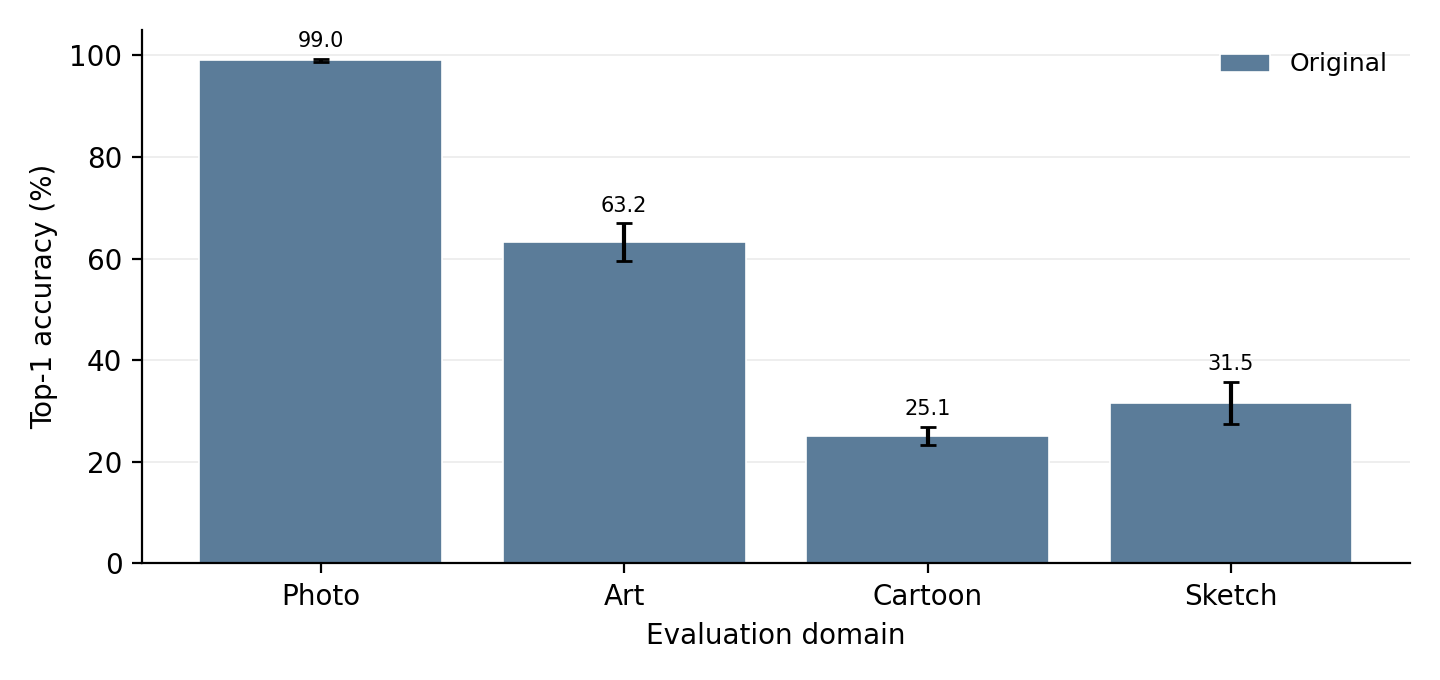
\includegraphics[width=\columnwidth]{figures/results_baseline.png}
\caption{Experiment 1: accuracy of the Original group on the in-domain Photo test set and on the three unseen target domains. Bars are means over three seeds; whiskers are standard deviations.}
\label{fig:results_baseline}
\end{figure}

%==================================================

\section{Progress/Current Status}
%==================================================

% TODO (Member 1): 4.1 material
% TODO (Member 2): 4.2 material
% TODO (Member 3): 4.3 material

% TODO (Member 4): 4.4 Training, Evaluation and Ablation Preparation — draft below

\subsection{Training, Evaluation and Ablation Preparation}
\label{sec:training_prep}

The unified training and evaluation code is in place and has been validated on the local PACS copy:

\begin{itemize}
\item \textit{Data verification.} All six project splits were validated against the local PACS copy: every referenced image exists, folder names match labels, per-split counts and class distributions match the recorded protocol (including sha256 verification of the split files), and no image appears in more than one split. The 9{,}990 usable images plus the one excluded ``ERROR'' image account for all files on disk.
\item \textit{Unified training pipeline.} One training script serves all three groups through fixed image manifests; the groups differ only in the manifest they read. Training is step-budgeted (660 optimizer steps for every group) so that the two augmented groups, which have twice the training images, do not receive more optimization.
\item \textit{Fairness checker.} A mechanical checker validates the fairness constraints of Section~\ref{sec:exp_design} on the two augmented manifests (same originals covered, same style pool hash, same counts, identical content--style pairing) before any augmented run is accepted. It also checks that no style image in the frozen pool is a PACS image, by comparing content hashes against the whole local PACS copy; this guards against test-set appearance entering training through the style pool. Finally it recomputes the training-configuration fingerprint from the full configuration recorded in each run summary and rejects any run whose hyper-parameters differ from the current ones. The checker was tested to pass on a correct pair of manifests, to reject a deliberately tampered pairing, to reject a pool built from PACS test images, and to reject a run recorded with a different step budget.
\item \textit{Experiment 1 (domain gap) completed.} The Original group was trained with three seeds on the fixed 660-step budget. It reaches $99.0\pm0.3\%$ on Photo Test but only $39.9\pm2.7\%$ averaged over the three unseen domains (Art Painting $63.2\pm3.7\%$, Cartoon $25.1\pm1.8\%$, Sketch $31.5\pm4.2\%$), as recorded in Table~\ref{tab:results}. The gap confirms the premise of the project, and the ordering of the three domains shows where augmentation has the most room to help.
\item \textit{Checkpoint-selection correction.} An initial protocol selected the checkpoint with the best Photo Validation accuracy. Because the validation set has only 150 images and its accuracy saturates at 97--98\% within 60 steps, this selection was effectively picking noise: it inflated the seed-to-seed spread of cross-domain accuracy to 7.22 points, compared with 2.71 points when the final checkpoint of the fixed budget is reported. We removed the selection step and now report the final checkpoint for every group and every seed, which also makes the protocol easier to reproduce.
\end{itemize}

% TODO (Member 5): 4.5, 4.6

%==================================================
\section{Next Steps and Plan for Completion}
%==================================================

% TODO (Members 3, 4): 5.3 Ablation and Analysis Plan material

% TODO (Member 4): \subsection{Experiment Completion Plan} — final text below

% Member 4 - Section 5.2 Experiment Completion Plan
\subsection{Experiment Completion Plan}
\label{sec:completion_plan}

The unified training and evaluation code is complete and validated on the local PACS copy, so the remaining experiment work is primarily GPU time. The plan below assumes the two generators are delivered by their owners in week 1; the frozen style pool they will use is already in place (Section~\ref{sec:exp_design}).

\begin{itemize}
\item \textit{Week 1: Experiment 1 and baseline replication.} \textit{Done.} The Original group has been run with seeds $\{0,1,2\}$ on the fixed 660-step budget, giving $99.0\pm0.3\%$ in-domain and $39.9\pm2.7\%$ cross-domain. The step budget was fixed before these runs (30 nominal passes over the training set). A diagnostic run to 1{,}320 steps, recorded but not used for tuning, shows that cross-domain accuracy fluctuates within a narrow band from the first evaluation onwards rather than improving systematically with more steps; the budget was therefore kept at 660 steps for all groups and every group reports its final checkpoint (Section~\ref{sec:resnet_baseline}). The remaining work in this week is to fix the checkpoint-selection policy, which we have done (Section~\ref{sec:resnet_baseline}), and to confirm the final protocol with the group.
\item \textit{Week 2: Experiments 2 and 3.} Generate the two augmented datasets from the frozen style pool and run +AdaIN and +Ours with the same three seeds. Run the fairness checker on both augmented manifests before training.
\item \textit{Week 3: Experiment 4 and ablation.} Sweep $\alpha \in \{0.25, 0.5, 0.75, 1.0\}$ for both methods on one seed, plus the $\beta$ sweep for the structure-preserving method; compute LPIPS and EdgeScore (Section~\ref{sec:evaluation_metrics}) on all generated datasets.
\item \textit{Week 4: Replication and analysis.} Re-run the best configurations on the remaining seeds, assemble per-domain and per-class tables, and identify where structure preservation helps or fails.
\end{itemize}

Compute budget: one training run takes roughly 10 minutes on the project GPU (RTX 4070 Laptop, 8\,GB), so the full plan above totals approximately 15--20 GPU-hours including sweeps and reruns, which fits the available hardware within the schedule.

% TODO (Member 5): 5.1, 5.4, 5.5

%==================================================
\begin{thebibliography}{00}

\bibitem{zhou2023dgsurvey}
K.~Zhou, Z.~Liu, Y.~Qiao, T.~Xiang, and C.~C.~Loy,
``Domain generalization: A survey,''
\textit{IEEE Trans. Pattern Anal. Mach. Intell.}, vol.~45, no.~4, pp.~4396--4415, 2023.

\bibitem{zhou2021mixstyle}
K.~Zhou, Y.~Yang, Y.~Qiao, and T.~Xiang,
``Domain generalization with MixStyle,''
in \textit{Proc. Int. Conf. Learning Representations (ICLR)}, 2021.

\bibitem{huang2017adain}
X.~Huang and S.~Belongie,
``Arbitrary style transfer in real-time with adaptive instance normalization,''
in \textit{Proc. Int. Conf. Computer Vision (ICCV)}, 2017.

\bibitem{li2017dg}
D.~Li, Y.~Yang, Y.-Z.~Song, and T.~Hospedales,
``Deeper, broader and artier domain generalization,''
in \textit{Proc. Int. Conf. Computer Vision (ICCV)}, 2017.

\bibitem{zhou2020dassl}
K.~Zhou, ``Dassl: Domain adaptation and generalization library,''
\url{https://github.com/KaiyangZhou/Dassl.pytorch}, accessed 2026.

\bibitem{he2016resnet}
K.~He, X.~Zhang, S.~Ren, and J.~Sun,
``Deep residual learning for image recognition,''
in \textit{Proc. IEEE Conf. Computer Vision and Pattern Recognition (CVPR)}, pp.~770--778, 2016.

\bibitem{zhang2018lpips}
R.~Zhang, P.~Isola, A.~A.~Efros, E.~Shechtman, and O.~Wang,
``The unreasonable effectiveness of deep features as a perceptual metric,''
in \textit{Proc. IEEE Conf. Computer Vision and Pattern Recognition (CVPR)}, 2018.

\bibitem{canny1986}
J.~Canny,
``A computational approach to edge detection,''
\textit{IEEE Trans. Pattern Anal. Mach. Intell.}, vol.~8, no.~6, pp.~679--698, 1986.

\bibitem{szegedy2016rethinking}
C.~Szegedy, V.~Vanhoucke, S.~Ioffe, J.~Shlens, and Z.~Wojna,
``Rethinking the inception architecture for computer vision,''
in \textit{Proc. IEEE Conf. Computer Vision and Pattern Recognition (CVPR)}, 2016.

\bibitem{loshchilov2017sgdr}
I.~Loshchilov and F.~Hutter,
``{SGDR}: Stochastic gradient descent with warm restarts,''
in \textit{Proc. Int. Conf. Learning Representations (ICLR)}, 2017.

\end{thebibliography}

\end{document}
